%%%%%%%%%%%%%%%%%%%%%%%%%%%%%%%%%%%%%%%%%
% Thesis 
% LaTeX Template
% Version 1.3 (21/12/12)
%
% This template has been downloaded from:
% http://www.latextemplates.com
%
% Original authors:
% Steven Gunn 
% http://users.ecs.soton.ac.uk/srg/softwaretools/document/templates/
% and
% Sunil Patel
% http://www.sunilpatel.co.uk/thesis-template/
%
% License:
% CC BY-NC-SA 3.0 (http://creativecommons.org/licenses/by-nc-sa/3.0/)
%
% Note:
% Make sure to edit document variables in the Thesis.cls file
%
%%%%%%%%%%%%%%%%%%%%%%%%%%%%%%%%%%%%%%%%%

%----------------------------------------------------------------------------------------
%	PACKAGES AND OTHER DOCUMENT CONFIGURATIONS
%----------------------------------------------------------------------------------------

\documentclass[11pt, a4paper, oneside]{Thesis} % Paper size, default font size and one-sided paper

%\graphicspath{{./Pictures/}} % Specifies the directory where pictures are stored



\begin{document}

%----------------------------------------------------------------------------------------
%	TITLE PAGE
%----------------------------------------------------------------------------------------

\begin{titlepage}
\begin{flushleft}
\Large{
\univname\\
\instname\\
\deptname
}
\end{flushleft}
\begin{center}


\vspace{1cm}


\includegraphics[width=0.4\linewidth]{./figures/miskolc_logo}

\vspace{1cm}

{\huge \bfseries \ttitle}\\[0.4cm] % Thesis title

\textsc{\Large \degreename}\\[0.5cm] % Thesis type
 
 \vspace{5cm}

\textit{Author:}\\
\authornames\\
\textsc{\authorId}
 
\vspace{2cm}

\textit{Supervisor}\\
\supname

\vspace{2cm}

\textbf{\the\year.}
%\includegraphics{Logo} % University/department logo - uncomment to place it
 
\vfill
\end{center}

\end{titlepage}

%----------------------------------------------------------------------------------------
%	DECLARATION PAGE
%	Your institution may give you a different text to place here
%----------------------------------------------------------------------------------------

\thispagestyle{empty}
\phantomsection
\addcontentsline{toc}{chapter}{Szerzői Nyilatkozat}
%\null
%\vfil
%\vskip 60\p@
\begin{center}{\huge\bf Szerző Nyilatkozat\par}\end{center}


Igazolom hogy tényleg én írtam ezt a művet bla bla bla...

Miskolc, \today \\

\vspace{2cm}
\begin{minipage}{0.4\textwidth}
\begin{center}
\rule{5cm}{0.5mm} \\
\authornames
\end{center}
\end{minipage}

\clearpage % Start a new pag

\tableofcontents
\newpage

\chapter{Introduction.}
\label{chap:introduction}

Providing a filter to accurately predict and remove noise from measurements is a very active research area.
The Horus system showed that using time series instead of single values increases efficiency.
Filters can be applied as preprocessing algorithm to a WLAN to make steady connection to an Access Point.
Analysis of time series of WiFi RSSI measurements could lead to the development of an efficient client site filtering method for indoor positioning systems.
There are various time series filtering methods in the literature. This paper focuses only on two simple solution which are based on time windowing.
In the case that the two filters work efficiently, the process could be applied to networks with different filters to reach an optimal solution.
Computational complexity also gives an important constrain of these filtering methods, because the client devices usually have limited computational capacity and battery life.

\section{ILONA}
The presented results are connected to the Indoor Positioning Research at the University of Miskolc. The ILONA System is web application for indoor positioning. It provides positioning functions for client. 
ILONA stands foor  INdoor LOcation and NAvigation which is a web application
created to perform indoor positioning and navigation tasks.
It is made up by loosely coupled components such as \texttt{measurement, positioning, navigation} and \texttt{tracking}.
This paper focuses on the data analysis and data mining of the ILONA System.
A proper client side filtering method could increase the performance and the accuracy of the positioning service of the ILONA System.


\chapter{Related Works}
\label{chap:relatedWorks}
This chapter presents the basic concepts  of indoor postioning systems the most widely used technologies and gives a brief overview of the mathematical background of modeling and filtering  time serries.
\section{Indoor Positioning}
The first Indoor positioning systems were planned in the 1980s but they become popular in the last decade \cite{liu2007survey,gu2009survey}. 
IPS systems can be used in hospitals, malls, airports and offices.
Indoor positioning is challenging due to the unique properties of the indoor environment.
GPS is a very popular method of position, however it is not suited for such tasks because of its line of sight requirements and the multipath effect.
Wireless LAN, Bluetooth, infrared, ultrasonic and radio frequency  technologies are the most popular.
Active Badge \cite{want1992active} was the first indoor positioning system which was based on infrared signals.
Fingerprinting methods were first presented by the RADAR system \cite{bahl2000radar}.
RFID \cite{ni2004landmarc} based technologies has emerged in the last years.
Hybrid Indoor Positioning Systems \cite{baniukevic2013hybrid} has been created in the least few years.
This paper connects to the ILONA System which is a hybrid indoor positioning and naviagtion framework. \cite{ZsoltToth2015}.


\subsection{Indoor Positioning with Wireless LAN}
	Wireless LAN(WLAN) was designed to transmit data wirelessly over small distances, and connecting to the internet. WLAN also can be used for indoor positioning purposes [8]. \cite{evennou2006advanced}. WLAN is highly available since most devices can receive and process WLAN signals, smart phones can be programmed easily so they can implement client side filtering methods. It is also very cost-effective since the data received is highly accurate in most situations. Received Signal Strength Indication is measured by the device and it is determined for each available Access Points.
	 WLAN positioning is based on the measurement of the signal strength value (RSSI). The user  is linked to or or multiple Access Points(AP) to determine user location at any given time. The User has to have a relatively stable and continuous connection. Unfortunatelly, the RSSI signal is not stable. It fluctuates over time even without any environmental impact. This fluctuation can be filtered at client side Electromagnetic signals are reflected \cite{kjaergaard2012mobile} by most bodies, as it can be seen on Figure \ref{fig:kockahaz}.
	\begin{figure}[h]
		\centering
		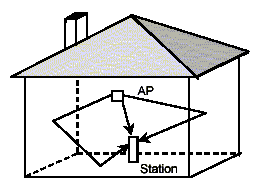
\includegraphics[width=.3\linewidth]{figures/Reflect.png}
		\caption{Indoor WLAN signal reflection \cite{Reflections}}\label{fig:kockahaz}
	\end{figure}
	 A few people in a room can drastically alter the measurements, making it less reliable the more reflective bodies there are in the room. 

\subsection{Fingerprinting Methods}
	Although WLAN was not developed to be a positioning system, it is a popular candidate for indoor positioning systems.  Most of the existing solutions are based on the fingerprinting technique \cite{kaemarungsi2004properties}\cite{honkavirta2009comparative}  Instead of determining the distance between the AP and the user by the  RSSI, it creates a radio map.Fingerpringint based indoor positioning methods require huge computational capacity, so they can be performed only on the server side.
	
\subsection{WiFi Based Solutions}
WiFi \cite{chen2002signal}based positioning popular due to the spread of mobile and smart phones in the early 2000's. However, GPS and AGPS are availeble in the modern phones, these technologies cannot be used in indoor environment. As more buildings, like hospitals, malls, etc. are designed with indoor WiFi Access Points in mind, it is only natural to try and use these APs to determine location.
\subsection{Horus System}
The Horus\cite{youssef2005horus} system is location determining system based on the IEE 802.11b WiFi , and Bluetooth connection, as seen on \ref{fig:horusimage}.The system determines user location by the received RSSI values from the access points. RSSI values are sent automatically, so implementing the system is purely a software solution, requiring no modifications on the hardware.Server oldalon van implementalva itt is a szamitas, de a kliens oldali szures novelte a hatekonysagot.
\begin{figure}[!h]
	\centering
		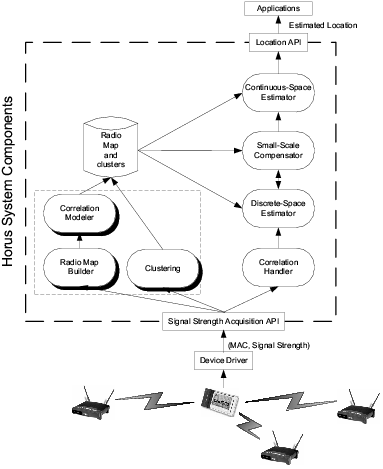
\includegraphics[width=.55\linewidth]{figures/Horus.png}
		\caption{Horus System \cite{HORUS}}\label{fig:horusimage}
\end{figure}


\section{Time Series Filtering Methods}
\subsection{Time Series}
Time series \cite{kalman1960new}\cite{durbin2012time} is a set of observations (x), being recorded a specified time (t).
It is stochastic in a sense that most of the time, measurements closer together have more importance towards each other.
Time series are often plotted with line charts on a one dimensional panel, as they represent the data fluctuations well.
They are very frequently used in most domain of applied science.

\subsection{Discrete Time Series}
A discrete time series is one which the set $T_0$ of times at which observations are made is a discrete set, for example being recorded at fixed time intervals. It is called continuous, if the measurements are being recorded continuously over a set amount of time.
\subsection{ARMA Models}
The three main modelling variations of importance are the autoregressive(AR),
moving average (MA), and the integrated (I) models. The ARMA modelling of wifi rssi will be the topic of a future research.


AR(p) refers to the autoregressive model of order p
$$ 
X_t = c + \sum_{i=1}^p \varphi_i X_{t-i}+ \varepsilon_t .\, 
$$
where $\varphi_1, \ldots, \varphi_p$ are parameters, c is a constant, and the random variable $\varepsilon_t$ is white noise.

Some constraints are necessary on the values of the parameters so that the model remains stationary. For example, processes in the AR(1) model with $|\phi_1| \geq 1$ are not stationary.

The notation MA(q) refers to the moving average model of order q:
$$
X_t = \mu + \varepsilon_t + \sum_{i=1}^q \theta_i \varepsilon_{t-i}\,
$$
where the $\theta_1, ..., \theta_q$ are the parameters of the model, $\mu$ is the expectation of $X_t$ (often assumed to equal 0), and the$ \varepsilon_t, \varepsilon_{t-1},...$ are again, white noise error terms.


The notation ARMA(p, q) refers to the model with p autoregressive terms and q moving-average terms. This model contains the AR(p) and MA(q) models,
$$
X_t = c + \varepsilon_t + \sum_{i=1}^p \varphi_i X_{t-i} + \sum_{i=1}^q \theta_i \varepsilon_{t-i}.\,
$$
The general ARMA model was described in the 1951 thesis of Peter Whittle, who used mathematical analysis (Laurent series and Fourier analysis) and statistical inference.


\subsection{Filtering Methods}
Filtering is the method of separating the noise from the signal, prediction of future values and control of current and future values.


\subsection{Time Windowing}
Time windowing is the process of allowing certain methods to stay idle for a certain amount of time before continuing to run or terminate. This certain amount of time depends on the predefined amount, and can be modified in the code. It is purely a software solution on most cases.In most cases, programs cannot andvence without any imput. Introducing a time window can make the program dynamic, because it can respond if it doesn't receive the needed values.

\chapter{Filtering Methods}
\label{chap:filteringMethods}
The goal of the following filters are to reduce caused by  multiple factors. These distractions are hard to avoid, and there is no surefire way to get rid of them. Filtering aims to solve this problem by creating an algorithm to reduce noise as much as possible, as simply as possible.


The unfiltered RSSI values, on shown on a diagram:
\begin{figure}[!h]
	\centering
		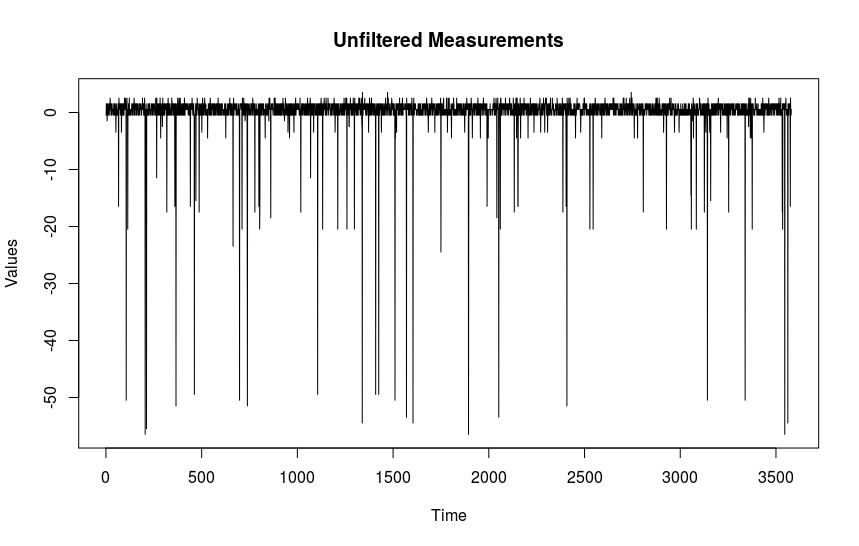
\includegraphics[width=.9\linewidth]{figures/UnfilteredZeroV1.png}
		\caption{RSSI values \cite{HORUS}}\label{fig:UnfilteredZero}
\end{figure}

And a summary of the values:
$$
\begin{array}{cccccc}
Min.& 1st Qu. & Median & Mean & 3rd Qu. & Max.\\
-87.00 & -31.00 & -30.00 & -30.53 & -29.00 & -27.00
\end{array}
$$
\section{Formal Description}
\subsection{First Filter}
The first one's mathematical model:
$y=(y_1,y_2\ldots y_n)$ is the filtered vector,$x=(x_1,x_2,\ldots x_n)$ is the starting value vector $ n\in \mathbb{N} $ is the number of values in the vector and $m \in \mathbb{N}$ is the memory size.
\begin{equation}\fontsize{15pt}{2}
y=(h(x,1,m),h(x,2,m)\ldots h(x,m,m), f(x,m+1,m)\ldots f(x,n,m))
\end{equation}
Where
\begin{equation}\fontsize{15pt}{2}
h(x,i,m)={(\sum\limits_{j=i}^{i+m-1}x_i) \over m}
\end{equation}
And
\begin{equation}\fontsize{15pt}{2}
f(x,i,m)=
\left\{
	\begin{array}{ccc}
	x_i & \mbox{if} |x_i-x_{i-1}|<t \\
	\\
	\overline{(x_i\ldots x_{i-m})} & \mbox{if} |x_i-x_{i-1}|>t
	\end{array}
\right.
\end{equation}           
The first part(h(x,i,m)):


The algorithm follows a simple pattern for the first 5 values. It takes the average from $x_i\ldots x_{i+m}$ indexes to create the filtered value of $y_1\ldots y_m$.
After the first m elements are calculated, it uses a different $f$ function to calculate the rest of the elements of y. 


The second  part(h(x,i,m)):

After the first 5 elements, the algorithm's actions are determined by a t variable.
If t is lesser than $|x_i-x_{i-1}|$, so the difference between the current and the last element exceeds the value of t:

the average of the last 5 $x$ value is put into the current y element.
If the previous condition is false, then the current x element is used as the filtered value.



\subsection{Second filter}
The second one's mathematical model:
$y=(y_1,y_2\ldots y_n)$ is the filtered vector,$x=(x_1,x_2,\ldots x_n)$ is the starting value vector $ n\in \mathbb{N} $ is the number of values in the vector and $m \in \mathbb{N}$ is the memory size.
The second filter's algorithm is much like the first one, except t is calculated after every iteration: 


\begin{equation}\fontsize{15pt}{2}
t=\sqrt{{1\over m}\sum\limits_{j=i}^{i-m}(x_j-\overline{x})^2}
\end{equation}



The second pard of the algorithm is different: 

The f function determines the elements by calculating a $t$ threshold that changes dynamically through the the function. It is always calculated by taking the standard deviation of the last 5 elements of the unfiltered vector. After the algorithm knows the value of t, it checks if the difference between the current element and the last element is greater than this value.

In the case that it is, it takes the average of the last m elements of the $X$ vector and puts it in the $y_i$ element.

If it's lesser then the t value, then $x_i$ is imply put into $y_i$.





\section{R Implementation} 
The implementations of the mathematical descriptions were done in R script.
The two filters are similar in nature, although offering different results.
The end results differ mildly depending on the choosing of threshold and memory size.
Choosing those two variables is key to an optimal filtering.
\subsection{First filter implementation}
The algorithm -- **
\begin{figure}[h!]
\fontsize{14}{2}
	\begin{lstlisting}
while(j<=memsize)
{
  i=1;
  while(i<=memsize)
  {
    a[i]<-Measurement$Signal[i+j-1]
    i=i+1
  }
  FilteredMeasurement$Signal[j]<-mean(a)
  j=j+1
}
	\end{lstlisting}
	\caption{The h(x,i,m) function, implemented.}\label{fig:code}
\end{figure}
\begin{figure}[h!]
\fontsize{14}{2}
	\begin{lstlisting}
while(x<=nrow(Measurement))
{
    if((abs(Measurement$Signal[x]-Measurement$Signal[x-1]))>thr)
    {
      i=1;
      while(i<=memsize)
      {
        a[i]<-Measurement$Signal[x-memsize+1+i]
        i=i+1
      }
      FilteredMeasurement$Signal[x]<-mean(a)
    }
    else
    {
      FilteredMeasurement$Signal[x]<-Measurement$Signal[x]
    }
  x=x+1
}
	\end{lstlisting}
	\caption{The f(x,i,m) function, implemented.}\label{fig:code}
\end{figure}

The following diagram and summary is after the filtering, with t and m chosen as 5:
\begin{figure}[h!]
	\centering
		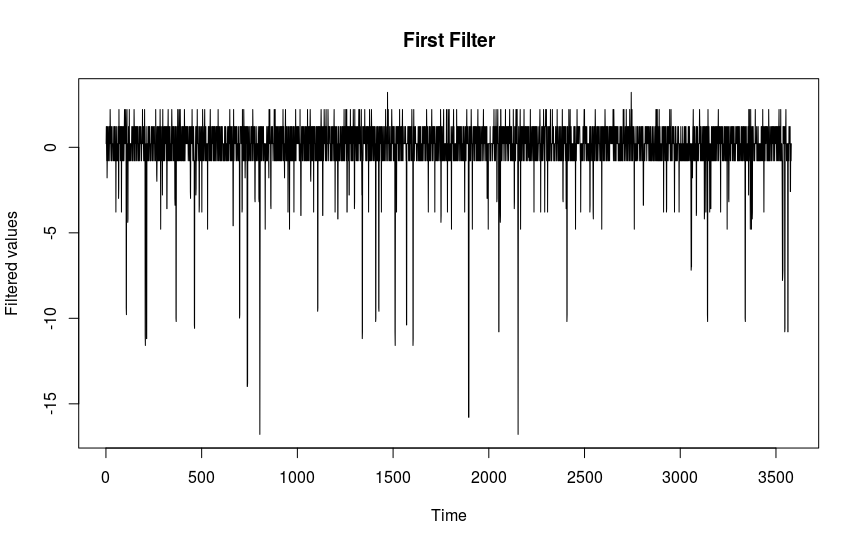
\includegraphics[width=.9\linewidth]{figures/FirstFilterZeroV1.png}
		\caption{Values with the first filter \cite{FirstFilter}}\label{fig:FirstZero}
		
		$$
		\begin{array}{cccccc}
		Min.& 1st Qu. & Median & Mean & 3rd Qu. & Max.\\
		-47.00 & -31.00 & -30.00 & -30.21 & -29.00 &   -27.00 
		\end{array}
		$$
		         
		
\end{figure}
\subsection{Second filter implementation}
Since the first part of the algorithm is analogous with the first one, it will not be included in this section.
The second part of the implementation is as follows:
\begin{figure}[h!]
\fontsize{14}{2}
	\begin{lstlisting}
while(x<=nrow(Measurement))
{
  thr<-(sd(a))*3
  i=1;
  while(i<=memsize)
  {
    a[i]<-Measurement$Signal[x - memsize + i]
    i=i+1
  }
  
  if((abs(Measurement$Signal[x]-Measurement$Signal[x - 1]))>thr)
  {
    FilteredMeasurement$Signal[x]<-mean(a)
  }
  else
  {
    FilteredMeasurement$Signal[x]<-Measurement$Signal[x]
  }
  x=x+1
}

	\end{lstlisting}
	\caption{The f(x,i,m) function, implemented.}\label{fig:code}
\end{figure} 


The following diagram and summary is after the filtering, with m chosen as 5:


\begin{figure}[h!]
	\centering
		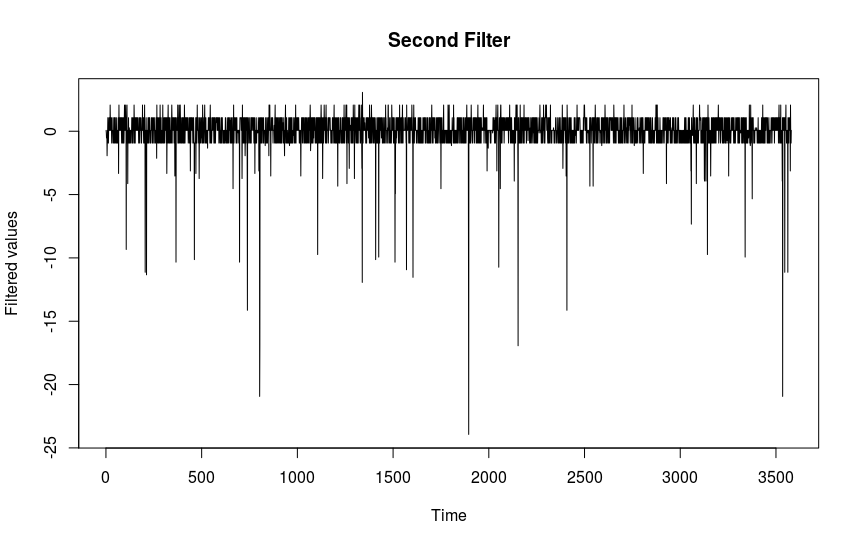
\includegraphics[width=.9\linewidth]{figures/SecondFilter.png}
		\caption{Values with the second filter \cite{secondzero}}\label{fig:SecondZero}
\end{figure}


\begin{figure*}
$$
		\begin{array}{cccccc}
		Min.& 1st Qu. & Median & Mean & 3rd Qu. & Max.\\
		-54.00 & -31.00 & -30.00 & -30.07  & -29.00 &-27.00 
		\end{array}
		$$
\end{figure*}
		          
		   
\chapter{Evaluation}
\label{chap:evaluation}

\section{Comparison}

\section{Suggestion}
\chapter{Summary}
\label{chap:summary}

The research surrounding the active filtering of data sets is a very popular topic today, and for a good reason.
This paper proves that preprocessing filters can be a very effective tool in indoor positioning research and generally increasing WLAN signals.
Even using using a simple, time windowing program can increase signal strength and accuracy by a margin, which proves that implementing more filters could result in an optimal method.


\appendix

\chapter{CD Melléklet}

Lorem ipsum dolor sit amet, consectetuer adipiscing elit, sed diam nonummy nibh euismod tincidunt ut laoreet dolore magna aliquam erat volutpat. Ut wisi enim ad minim veniam, quis nostrud exerci tation ullamcorper suscipit lobortis nisl ut aliquip ex ea commodo consequat. Duis autem vel eum iriure dolor in hendrerit in vulputate velit esse molestie consequat, vel illum dolore eu feugiat nulla facilisis at vero eros et accumsan et iusto odio dignissim qui blandit praesent luptatum zzril delenit augue duis dolore te feugait nulla facilisi. Nam liber tempor cum soluta nobis eleifend option congue nihil imperdiet doming id quod mazim placerat facer possim assum. Typi non habent claritatem insitam; est usus legentis in iis qui facit eorum claritatem. Investigationes demonstraverunt lectores legere me lius quod ii legunt saepius. Claritas est etiam processus dynamicus, qui sequitur mutationem consuetudium lectorum. Mirum est notare quam littera gothica, quam nunc putamus parum claram, anteposuerit litterarum formas humanitatis per seacula quarta decima et quinta decima. Eodem modo typi, qui nunc nobis videntur parum clari, fiant sollemnes in futurum.

\bibliographystyle{plain}
\bibliography{references}

\end{document}